\documentclass{article} % For LaTeX2e
\usepackage{nips13submit_e,times}
\usepackage{hyperref}
\usepackage{url}
\usepackage{graphicx}
\usepackage{wrapfig}
\usepackage{caption}
\usepackage{subfig}
\usepackage{adjustbox}

\captionsetup{
  font=footnotesize,
  justification=raggedright,
  singlelinecheck=false
}

\title{Banishing the Bid Bot: Detecting Online Bidding Fraud in Facebook Auctions \\ \large Team Random Clique}

\author{
Daniel Geng \\
504588536 \\
Department of Computer Science\\
University of California, Los Angeles\\
\texttt{danielgeng@cs.ucla.edu} \\
\And
Meghana Ginjpalli \\
804588573 \\
Department of Computer Science \\
University of California, Los Angeles\\
\texttt{mginjpalli@ucla.edu} \\
\AND
Sara Melvin \\
004590481 \\
Department of Computer Science \\
University of California, Los Angeles\\
\texttt{sara.melvin@gmail.edu} \\
\And
Sonu Mishra \\
604590548 \\
Department of Computer Science\\
University of California, Los Angeles\\
\texttt{skmishra@cs.ucla.edu} \\
\And
Andrew Wong \\
104036702 \\
Department of Computer Science\\
University of California, Los Angeles\\
\texttt{anjuwong@ucla.edu} \\
}

\newcommand{\fix}{\marginpar{FIX}}
\newcommand{\new}{\marginpar{NEW}}

\nipsfinalcopy % Uncomment for camera-ready version

\begin{document}

\maketitle

\begin{abstract}

The ubiquity of social media has made it an attractive platform for commercial advertisement.
To take advantage of this, Facebook places its web ``real estate" on sale to businesses through auctions.
Many of the bidders are bots, making it nearly impossible for human users to win any auctions.
The problem statement from the Kaggle competition ``Facebook Recruiting IV: Human or Robot?" was to identify as many bots as possible.
In this project, we implement various anomaly detection approaches, including classic machine learning models and a Bayesian-based model, BIRDNEST.
Our approaches are then compared and contrasted with the Kaggle competition winner.
Various pre-processing methods of the input features are analyzed and tested to discover the best indicators that classify a user as a bot.
For evaluation, the ROC AUC score was used.
With BIRDNEST, we achieved a 0.8456 AUC score and with machine learning models, we achieved a 0.9169 AUC score using gradient boosting.

\end{abstract}

\section{Introduction}

Facebook is a popular online social media platform connecting users from all around the world.
Because of its high traffic, Facebook is an ideal form of commercial advertisement.
Businesses are able to reach out to their existing customers as well as advertise to new customers by specifying which group of users they would like to advertise to.
Although Facebook can provide space on both their website and mobile site, there is limited webpage ``real estate".
Therefore, Facebook sets up auctions for businesses to bid on designated spaces for advertisement purposes.

Facebook advertisement space is becoming increasingly sought after causing greater competition in Facebook bidding.
Unfortunately, legitimate businesses or organizations are being frustrated by bots as they bid at the last possible second. This practice is known as auction sniping which is often times implemented by a bidder's local software or by an online sniping service \cite{auction}.
Automated bids from bots are unfairly able to submit bids almost instantaneously, making it difficult for legitimate businesses to win auctions.

As more and more businesses are using bots to outbid each other, Facebook is trying to gain back trust of their bidders to keep their advertisement space highly desired. Existing approaches have been implemented in order to determine these anomalous users.
Thus, there is a lot of motivation for these companies to have some type of anomaly detector for removing these bots. 

``Facebook Recruiting IV: Human or Robot?" was a past Kaggle Competition that ended in June 2015.
The competition tackles the problem of bot detection in Facebook Ads bidding.
Our goal is to detect bot-user anomalies in this bidding environment using various anomaly detection methods.
In Section 2, we discuss previous related work in the area of online user anomaly detection and their advantages and disadvantages. In Section 3, we give an overview of our project approach. In Section 4, we discuss the Kaggle data used in this project. Section 5 goes over various software tools used for our project. Section 6 exhibits the results of the various algorithms and approaches we implemented. Lastly, Section 7 concludes with a discussion of our results.

\section{Related Work}

There are several types of approaches for user anomaly detection such as group-based, temporal-based, and edge attribute graph-based.

\subsection{Group-based Approach}

This approach aims to detect groups of anomalies based on features across multiple users.
Previous methods have attempted to classify based on the similarity of feature groups \cite{ndsync}.
Other methods detect group based anomalies by determining groups based on closeness of certain features, and then determining which groups are anomalous \cite{glad}.
The benefits of using these group-based approaches is that it uses the sheer amount of data provided to its advantage.
Generally, however, these approaches assume a static model for the data.
Additionally, due to the large amount of data processed by these approaches, the methods are computationally expensive.

\subsection{Temporal-based Approach}

Unlike some of the other approaches, this method uses only one feature to detect bot-users suspicious activity.
The temporal-based approach operates under the assumption that the time between user events for bots is significantly different behavior than normal users \cite{birdnest} \cite{rsc} \cite{sfp} \cite{cicp}.
This assumption holds in most situations.
However, bots could be compromised users, which camouflages the anomalous temporal feature(s) with their human host.
Therefore, other features may need to be used for improved detection of bot-users.

\subsection{Edge-attributed Graph-based Approach}

Conventional graph-based approaches observe topological patterns of relations between entities (i.e. users, products, etc), but do not leverage the edge-attributes.
The algorithm proposed in EdgeCentric utilizes more features by representing the relationship between entities as an edge-attributed multigraph \cite{edgecentric}.
Given the distribution of various clusters of benign user behavior, the information required to describe the behavior of a new user is found in terms of its minimum description length (MDL) from the clusters.
The MDL is used to compute how suspicious a certain user is.
The strength of this approach, however, relies on the rating relationship between users, products, and buyers.
In the project's bidding data, a seller and rating information is not disclosed, which potentially weakens the applicability of this approach.

\section{Approach}

The approach to this project is to compare and contrast various algorithms with different features to see which results in the best performance. From our research on user anomaly detection algorithms, we identified with BIRDNEST as a good approach to take because it estimates our beliefs about the user's behavior characteristics and captures our uncertainty about user behavior to determine suspiciousness. We adapted this to the bidding environment as a pure temporal approach. Additionally, we wanted to apply classic machine learning algorithms with various spatial and temporal features. We implemented the following algorithms: Support Vector Machines, Logistic Regression, Adaboost, Gradient Boosting, Random Forests, Bagging, and Extra Trees. 
Because the dataset from Kaggle (\url{https://www.kaggle.com/c/ facebook-recruiting-iv-human-or-bot/data}) provides labeled data, we decided to focus on these supervised algorithms for detection.
We used k-fold cross validation and tuned our hyperparameters evaluation metrics. 

To evaluate the efficacy model, we applied he trained model to our testing data and compared the classifying algorithms based on performance.
The metrics we will use to evaluate the performance of our algorithms is the area under the ROC curve (AUC). 

\section{Data}

The data provided includes timestamps of bids, merchandise categories, bidding devices, countries of bids, and the reference URL for a bid.
We used these features and state-of-the art anomaly detection algorithms to determine which method will best identify bot-users.

The bidder dataset contained approximately 2,000 instances and had the following features: bidder\_id, payment\_account, address, outcome.
The bid dataset contained approximately 7.6 million instances and had the following features: bid\_id, bidder\_id, auction, merchandise, device, time, country, ip, url.

The training data set provided by Kaggle had labels for each user, classifying each individual as a human or a bot.
However, the testing data had no labels; therefore, only the training data set could be used for training, validation, and testing.

The training data set was joined with the bids data set, resulting in over 3 million bids.
Overall, it contained 1,984 distinct bidders with 103 of the total users classified as bots.

\section{Software Tools}

Python was used for a majority of our data processing, given the large number of libraries that are publicly available.
Sklearn has a number of built-in machine learning algorithms.
Numpy is very useful for working with matrices and different feature vectors.
Pandas has a high performance data analysis tool used to analyze large amounts of data.
Matplotlib facilitates data visualization, which will yield insights into how our data is related.


\section{Results}
\subsection{BIRDNEST}

BIRDNEST \cite{birdnest} is a Bayesian-based approach to anomaly behavior detection. This algorithm identifies anomalous users by implementing two phases. First the algorithm models user behavior distributions as a mixture model (BIRD model) to produce the posterior distributions of user behavior. It calculates a user's score by determining the negative log likelihood of the user's posterior distribution given the global distribution of the BIRD Model (NEST metric).

Originally, the algorithm was built to identify rating-fraud by observing two features: rating behavior and inter-arrival times between user activity. In the context of auction bidding, the rating behavior was not used, however the temporal feature aspect of the algorithm seemed similar to the given situation. Therefore, this algorithm was adjusted to be a purely temporal-based approach.
	
\subsubsection{Implementation}

\textbf{Features Extracted} 

\begin{enumerate}
\item Inter-arrival time (IAT) distribution - time between user's activity events
\item Response Time - time between the previous bidder's bid and the user
\end{enumerate}

For selecting features, the first hypothesis was that bots will act similarly in a bidding environment as in a rating environment. Originally, the BIRDNEST paper showed an early spike for rating-bot IATs compared to humans. It was theorized that the bidding bot would be activated by the bot-creator once it had a paying client and then would bid on as many auctions that fit the client's demographic as possible. This would be a sort of blanket-bidding which would lead to smaller IATs than humans.

For the IAT distribution, the IAT values were computed and binned in a log-based binning histogram with log-base of 2 resulting in 47 buckets. The IAT feature was calculated in a similar manner as the BIRDNEST authors performed in their source code (\url{www.andrew.cmu.edu/user/bhooi/ratings.tar}). There were adjustments made in the following: processing the data and data structures for storing and tracking features.

As seen in Figure 1, we did not end up seeing the dramatic early spikes as we were hoping but on average, the bots had a smaller IAT. We therefore adjusted the log-base to see more or less of a granularity of this distribution. Other log-bases were attempted but did not dramatically alter the distributions. Therefore, we chose a log-base of 2 to give us the most detailed histogram in the most reasonable processing time.

\begin{figure}[!htb]
\centering
\captionbox{Normalized true human IAT distribution (left) and true bot normalized IAT distribution (right)}{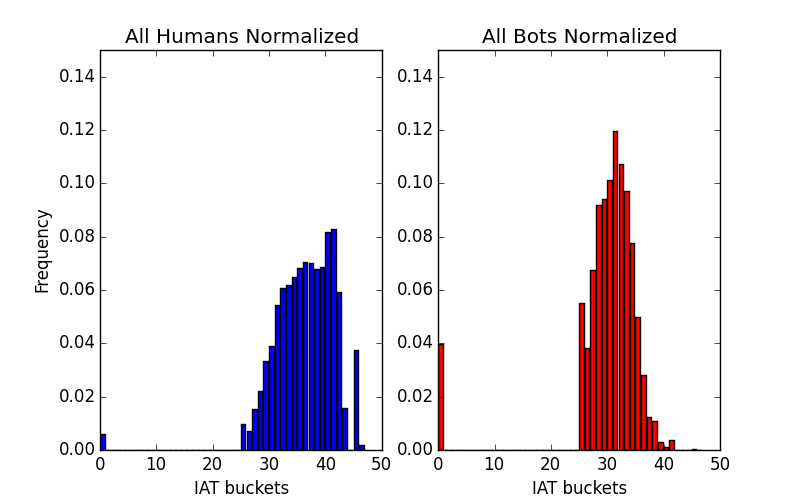
\includegraphics[scale=0.5]{img/bird_iat_dist.png}}
\end{figure}

After analyzing this feature we had another theory. Bot-creators activate their bots to be watchdogs on certain auctions paid for by their customers to outbid any competitive bid. This response time would then be smaller than a normal human's reaction time.

Upon searching for Kaggle winner blogs, the team came across the second place winner called the Small Yellow Duck (will be referred to later in this paper) who used, amongst other features, the median and mean response time of every bidder as a feature in her solution. To reflect this feature for better comparison to the professional's approach, the Small Yellow Duck's response times were extract and joined with a table consistent with the BIRDNEST format. The response time distribution was binned with the same log-base as IAT distributions which resulted in 44 buckets.

As shown in Figure 2, there is not a distinct distribution difference between these groups as originally hoped. This is because human users do not necessarily represent one person. Many human users in this data set have multiple people bidding with the same username on the same auctions. These multi-party users show very similar bot-like response times.

\begin{figure}[!htb]
\centering
\captionbox{Normalized true human response time distribution (left) and true bot normalized response time distribution (right)}{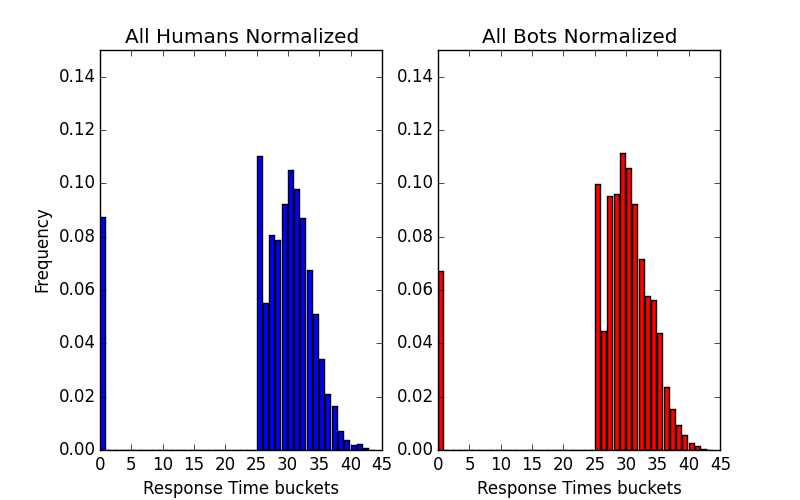
\includegraphics[scale=0.5]{img/bird_res_dist.png}}
\end{figure}

\subsubsection{Testing Methodology}

To test which features contribute the most, this algorithm was tested with just IAT as the only feature and then with both IAT and response time as features.

The BIRD mixture model is calculated by taking a random subset of each cluster's user distributions to estimate hyperparameters until convergence. Therefore, BIRDNEST results had a slightly varying AUC each time the model was run. Consequently, the algorithm was run with a varying cluster parameter, K (iterates from one cluster up to twenty clusters) to gain a true sense of the performance. Each user's score was averaged over these twenty runs and then re-ranked from highest to lowest. The true positive rate and false positive rate were calculated from this re-ranked list to produce the ROC curve and ultimately the AUC.

\subsubsection{Assumptions}

For the testing, the following assumptions were made:
\begin{itemize}
\item All users that did not have more than one bid in the data set were given zero IAT distributions.
\item All instances where a user bid more than once at the same time on the same auction with the same username were considered duplicates and only one of these instances was kept.
\end{itemize}

\subsubsection{Evaluation}

\textbf{Results: IAT only}

Despite not seeing the early spike as expected in the bot IAT distribution, using IAT as the only feature produced decent results.
Figure 3 shows the ROC with an AUC of 0.8415.

\clearpage

\begin{figure}[h]
\centering
\captionbox{BIRDNEST ROC curve of the average user scores over twenty different runs from one to twenty clusters, K, with only IAT as the feature.}
{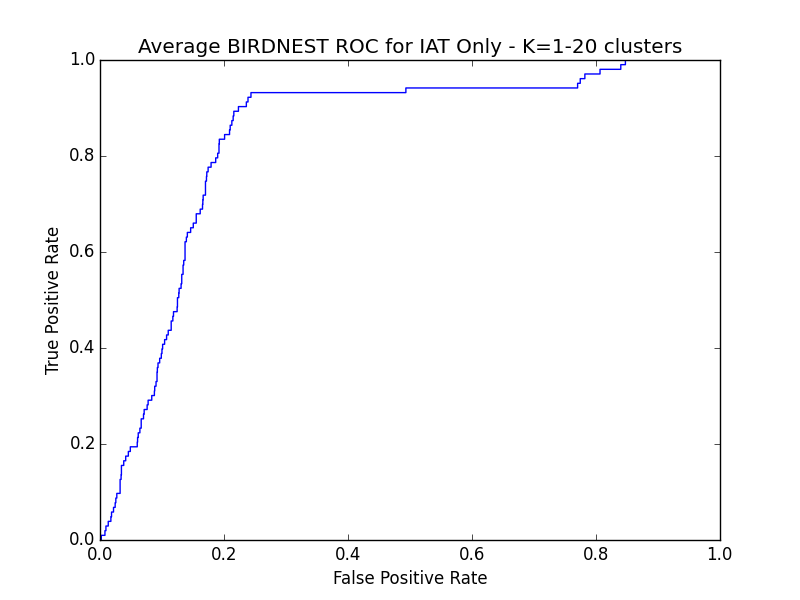
\includegraphics[scale=0.47]{img/bird_iat_roc.png}}
\end{figure}

Figure 4 shows the aggregated distributions of the first 103 users in the NEST score ranked list (right image in figure) and the rest of the ranked users (left image in figure). In comparing these distributions to Figure 1, it shows very similar results to BIRDNEST's top ranked distributions. This result shows that the BIRDNEST mixture model detects distributions that are anomalous to the rest of the normal distributions. However, the algorithm's performance decreases because our data consists of noise in the form of multi-party human users exhibiting bot-like behavior.

\begin{figure}[h]
\centering
\captionbox{BIRDNEST identified human IAT distribution (left) and BIRDNEST detected bot IAT distribution (right)} {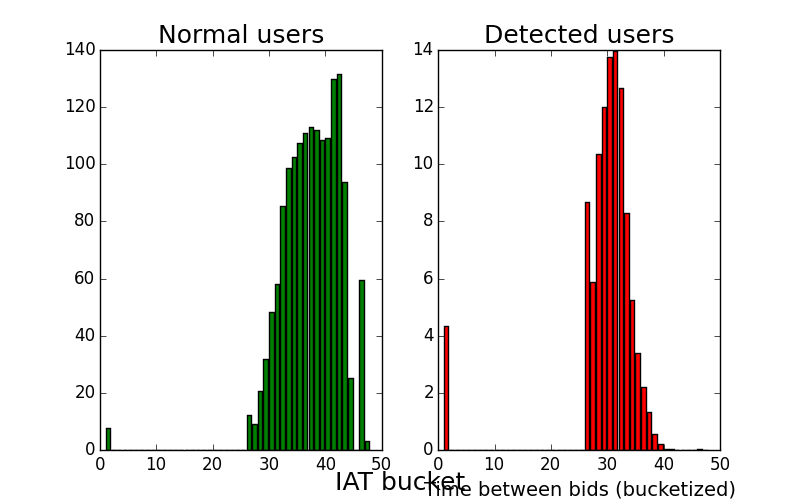
\includegraphics[scale=0.5]{img/bird_iat_pred.png}}
\end{figure}

\textbf{Results: IAT and Response Time}

Using Response Time and IAT distributions as features, the performance was only marginally improved.
Figure 5 shows the ROC with an AUC of 0.8456, which is only a 0.0041 improvement.

\clearpage

\begin{figure}[!htb]
\centering
\captionbox{BIRDNEST ROC curve of the average user scores over twenty different runs from one to twenty clusters, K, for response time and IAT features.}
{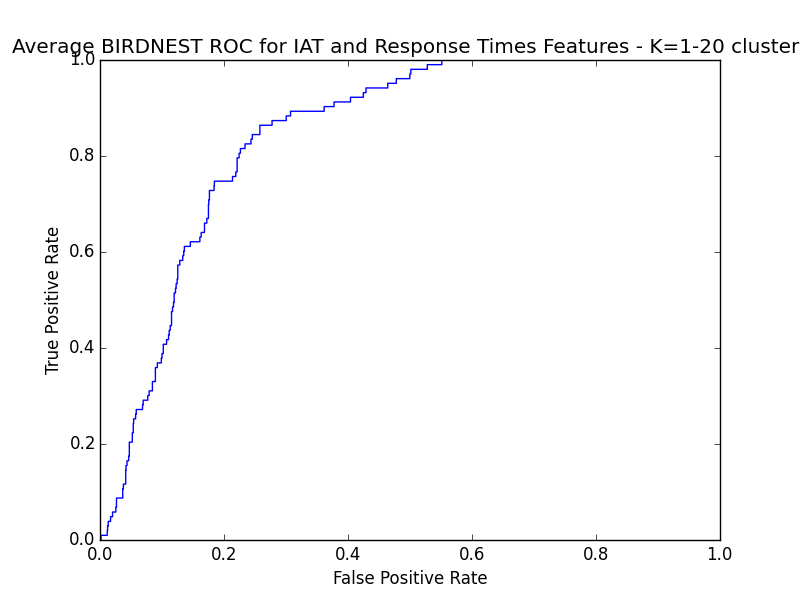
\includegraphics[scale=0.47]{img/bird_roc.png}}
\end{figure}

As mentioned previously, these multi-party users in the data set that exhibit bot-like behavior are a sort of noise in our data set. Therefore, we conclude that BIRDNEST is sensitive to noise and would work better in an environment where users are limited to have one person logged in at a time.

\subsection{Classic Machine Learning Approaches}

We implemented a variety of machine learning classification models and used various features to analyze which algorithm would result in the best performance.

\subsubsection{Implementation}

All machine learning models were implemented for binary classification, rather than a suspiciousness score.
Initially, support vector machines (SVMs) and logistic regression were implemented.
SVMs were tested with linear, polynomial, and radial kernels and logistic regression was tested using both primal and dual optimization functions.

However, because these models alone were not very effective, a myriad of boosting and ensemble methods were used in an attempt to improve performance.
The following methods were tested:

\begin{itemize}
\item Adaboost -- weights each classifier based on performance
\item Gradient boosting -- fits trees based on negative gradient of loss function
\item Random forests
\item Bagging -- trains on subsets of data and uses them to vote
\item Extra trees -- trains on subsets of data and averages them
\end{itemize}

All of these models fit numerous classifiers---typically decision trees---to make up for the shortcomings of the earlier classifiers.

\textbf{Features}

The given data was pre-processed in various ways.
A combination of the following features were tested in each model to varying degrees of performance.

\begin{itemize}
\item Log-bucketed IAT (base 2 and base 5) -- each bucket is a feature
\item Log-bucketed response time (base 2 and base 5) -- each bucket is a feature
\item Mean IAT
\item Mean response time
\item Total number of bids
\item Mean bids per auction
\item Number of devices
\item Number of IPs
\item Entropy of devices
\item Entropy of IPs
\end{itemize}

Initially, the consistently highest AUC was using only the IAT distributions which resulted in 0.87, however we wanted to see how much better we could make it.

Therefore, we derived a number of features from the given data.
First, we looked at the mean IAT and response times.
Another important feature turned out to be the number of bids and the number of bids per auction.
The total number of unique devices was also fairly important, and we also examined the number of unique IPs.
These additional features, in conjunction with the log-bins, was getting us around a 0.9 AUC.

The last features we explored were the entropies of the devices and IPs.
Our reasoning and the intuition behind this is was that the entropy values measure how distributed a user's IPs or devices are.
If the user posts from a single device only, there is little entropy.
However, if the user posts from a large number of devices with uniform frequency, the entropy is greater.

We tried this with numerous models that have the option to measure the Gini importance, and across the board, the new features we generated from the list above were higher than the binned distributions.
As we went along, we pruned them based on these importances, and we verified with performance to ensure that taking features out either improved or did not affect our model.

The following figures show the Gini importance of features for the gradient boosting classifier for all features and for the final set of features used.

\begin{figure}[h]
    \centering
    \subfloat[All features]{{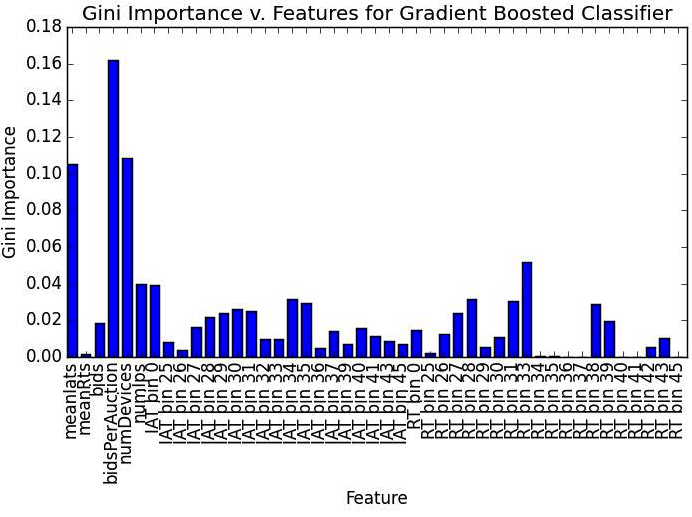
\includegraphics[width=6.56cm]{img/grad_gini_all.jpg} }}
    \qquad
    \subfloat[Final set of features]{{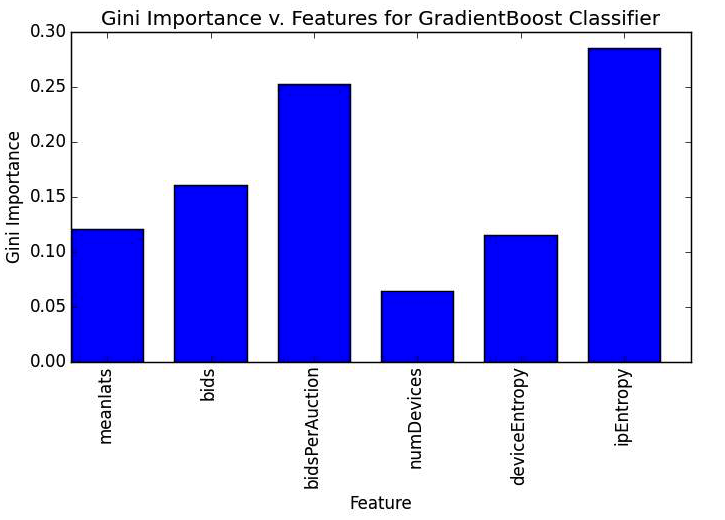
\includegraphics[width=6.5cm]{img/grad_gini.jpg} }}
\end{figure}

To find the optimal classifier for our features, we tried to sweep through different parameters for the original classification methods.
We tried to optimize $C$, the inverse regularization term, for each method.
A larger $C$ has less regularization and is more prone to overfitting.

For the ensemble methods, we also did a parameter sweep, varying the number of
estimators in the ensemble, or the number of boosting stages for certain models.
The models were cross-validated with an 80-20 partition of training and test
users. To ensure that our metrics stayed consistent, each model was trained on
the same partitions and the AUC scores were compared.

\subsubsection{Evaluation}

To evaluate overall performance, we used the AUC scores under the ROC curve.
The table below shows the AUC scores for the non-ensemble methods with various values of $C$.

\begin{adjustbox}{width=\textwidth,totalheight=\textheight,keepaspectratio}
\begin{tabular}{c|ccccccccccc}
Classifier & C=0.1 & 0.5 & 1 & 5 & 20 & 50 & 100 & 150 & 200 & 300\\
\hline
SVM (Linear) & 0.6829 & 0.7393 & 0.7566 & 0.7821 & 0.7964 & \textbf{0.8011} & 0.7932 & 0.7964 & 0.7891 & 0.7922\\
SVM (Poly) deg2 & 0.5455 & 0.5692 & 0.5972 & 0.6532 & 0.7077 & 0.7273 & 0.7286 & 0.7444 & 0.7277 & \textbf{0.7462}\\
SVM (Poly) deg3 & \textbf{0.6166} & 0.5402 & 0.5343 & 0.5841 & 0.5644 & 0.4730 & 0.5166 & 0.5305 & 0.5334 & 0.5596\\
SVM (Poly) deg4 & 0.5942 & \textbf{0.6124} & 0.6004 & 0.5542 & 0.5548 & 0.4949 & 0.4865 & 0.4894 & 0.4978 & 0.4779\\
SVM (Rbf) & 0.6340 & 0.6991 & 0.7179 & 0.7645 & \textbf{0.7996} & 0.7850 & 0.7847 & 0.7843 & 0.7813 & 0.7782\\
Log. Reg. (Primal) & 0.7360 & 0.7296 & 0.7333 & 0.7465 & 0.7677 & 0.7845 & 0.7968 & 0.8040 & 0.8086 & \textbf{0.8150}\\
Log. Reg. (Dual) & 0.7360 & 0.7296 & 0.7333 & 0.7466 & 0.7677 & 0.7846 & 0.7971 & 0.8047 & 0.8089 & \textbf{0.8164}\\
\end{tabular}
\end{adjustbox}

Somewhat surprisingly, SVMs were outperformed by logistic regression, and among
the SVMs tested, the best performance came with a linear kernel. Logistic
regression did have the best performance, but this was contingent on a high
value for $C$. The tables below show the AUC values for larger values of $C$ for
logistic regression with primal optimization. We noted that, as the value of $C$
was increased, the improvement gradually diminished. This behavior was expected,
as the value of $C$ is directly related to how overfit the model is, and if the
data is not separable, the performance for a single decision boundary is
limited.

\begin{tabular}{cccccccccc}
C=200 & 300 & 400 & 500 & 600 & 700 & 800 & 900 & 1000 \\
\hline
0.8021 & 0.8085 & 0.8126 & 0.8159 & 0.8183 & 0.8203 & 0.8218 & 0.8234 & 0.8246
\end{tabular}
\begin{tabular}{cccccccccc}
C=1200 & 1500 & 2000 & 3000 & 4500 & 7500 & 10000 & 15000 & 20000\\
\hline
 0.8267 & 0.8293 & 0.8324 & 0.8363 & 0.8392 & 0.8412 & 0.8423 & 0.8431 & 0.8441
\end{tabular}

In the ensemble methods, we found that, as expected, additional estimators did
not necessitate higher AUC scores. After performing a sweep over the number of
estimators, we concluded that, given our features, gradient boosting classifiers
perform the best. We performed this sweep using different sets of features, some
of which are shown in the tables below. We were guided by intuition gained from the Gini
importances to prune our features to select only those that mattered, and found
that not all features were beneficial to the model. The table below shows the
parameter sweep of the number of estimators using
all of the features we generated.

\begin{tabular}{c | c c c c c c c}
\# Estimators & 2 & 3 & 4 & 5 & 6 & 7 & 8\\
\hline
Adaboost & 0.8647 & 0.8658 & 0.8758 & 0.8817 & 0.8832 & 0.8822 & 0.8844\\
Gradient Boost & 0.8730 & 0.8780 & 0.8853 & 0.8855 & 0.8879 & 0.9008 & 0.8922\\
Random Forest & 0.7007 & 0.7464 & 0.7658 & 0.7771 & 0.7960 & 0.8078 & 0.8245\\
Bagging & 0.7092 & 0.7266 & 0.7614 & 0.7748 & 0.8018 & 0.7929 & 0.8087\\
Extra Trees & 0.7008 & 0.7478 & 0.7683 & 0.7829 & 0.7985 & 0.8139 & 0.8175\\
\end{tabular}
\begin{tabular}{c | c c c c c c c c }
\# Estimators & 9 & 10 & 15 & 30 & 50 & 100 & 150 & 200\\
\hline
Adaboost & 0.8874 & 0.8796 & \textbf{0.8881} & 0.8858 & 0.8763 & 0.8625 & 0.8586 & 0.8588\\
Gradient Boost & 0.9065 & 0.8964 & 0.9035 & \textbf{0.9115} & \textbf{0.9115} & 0.8973 & 0.9016 & 0.8919\\
Random Forest & 0.8276 & 0.8317 & 0.8420 & 0.8669 & 0.8867 & 0.8885 & \textbf{0.8900} & 0.8863\\
Bagging & 0.8200 & 0.8216 & 0.8399 & 0.8528 & 0.8703 & 0.8718 & 0.8786 & \textbf{0.8813}\\
Extra Trees & 0.8324 & 0.8364 & 0.8486 & 0.8770 & 0.8840 & 0.8904 & \textbf{0.8929} & 0.8921
\end{tabular}

The table below shows the parameter sweep of the number of estimators using only five
of the new features we generated: mean IAT, mean response time, number of bids,
number of bids per auction, and number of devices. In some cases, the models
outperforms their counterparts with all of the features. Although not strictly
better, this was still enough to give us a baseline for how good these new features are.

\begin{tabular}{c | c c c c c c c}
\# Estimators & 2 & 3 & 4 & 5 & 6 & 7 & 8\\
\hline
Adaboost & 0.8670 & 0.8801 & 0.8888 & 0.8888 & 0.8884 & \textbf{0.8911} & 0.8867\\
Gradient Boost & 0.8657 & 0.8805 & 0.8760 & 0.8963 & 0.8914 & 0.8939 & 0.8954\\
Random Forest & 0.6769 & 0.7176 & 0.7520 & 0.7559 & 0.7817 & 0.7798 & 0.8114\\
Bagging & 0.6980 & 0.7351 & 0.7582 & 0.7796 & 0.7944 & 0.7961 & 0.8107\\
Extra Trees & 0.6552 & 0.7065 & 0.7292 & 0.7612 & 0.7779 & 0.7953 & 0.7965
\end{tabular}
\begin{tabular}{c | c c c c c c c c}
\# Estimators & 9 & 10 & 15 & 30 & 50 & 100 & 150 & 200\\
\hline
Adaboost & 0.8875 & 0.8910 & 0.8823 & 0.8675 & 0.8644 & 0.8509 & 0.8523 & 0.8402\\
Gradient Boost & 0.8915 & 0.8971 & \textbf{0.9031} & 0.9021 & 0.8991 & 0.8893 & 0.8849 & 0.8790\\
Random Forest & 0.8051 & 0.8205 & 0.8523 & 0.8772 & 0.8758 & 0.8827 & \textbf{0.8906} & 0.8784\\
Bagging & 0.8208 & 0.8165 & 0.8419 & 0.8603 & 0.8815 & 0.8755 & \textbf{0.8854} & 0.8842\\
Extra Trees & 0.8057 & 0.8163 & 0.8343 & 0.8545 & 0.8721 & 0.8683 & 0.8742 & \textbf{0.8743}
\end{tabular}

The final set of features included were the following:

\begin{itemize}
\item Mean IAT
\item Number of bids
\item Number of bids per auction
\item Number of devices
\item Entropy of devices
\item Entropy of IPs
\end{itemize}

Using this set of features, we achieved the greatest average AUC score of
0.9169 using a gradient boosting classifier. The table below shows the AUC scores of the final set of features used with various number of estimators.

\begin{tabular}{c | c c c c c c c}
\# Estimators & 2 & 3 & 4 & 5 & 6 & 7 & 8\\
Adaboost & 0.8790 & 0.8892 & 0.8976 & 0.8996 & 0.9024 & 0.9022 & \textbf{0.9050}\\
\hline
Gradient Boost & 0.8918 & 0.8962 & 0.8990 & 0.9012 & 0.9029 & 0.9045 & 0.9059\\
Random Forests & 0.7081 & 0.7438 & 0.7767 & 0.7995 & 0.8152 & 0.8338 & 0.8325\\
Bagging & 0.7032 & 0.7482 & 0.7680 & 0.7882 & 0.8087 & 0.8128 & 0.8226\\
Extra Trees & 0.7050 & 0.7437 & 0.7710 & 0.7966 & 0.8130 & 0.8222 & 0.8288
\end{tabular}
\begin{tabular}{c | c c c c c c c c}
\# Estimators & 9 & 10 & 15 & 30 & 50 & 100 & 150 & 200\\
Adaboost & 0.9036 & 0.9004 & 0.9024 & 0.8967 & 0.8871 & 0.8773 & 0.8723 & 0.8684\\
\hline
Gradient Boost & 0.9071 & 0.9083 & 0.9129 & \textbf{0.9169} & 0.916 & 0.9090 & 0.8960 & 0.8864\\
Random Forests & 0.8481 & 0.8517 & 0.8756 & 0.8923 & 0.9024 & 0.9086 & 0.9105 & \textbf{0.9112}\\
Bagging & 0.8293 & 0.8384 & 0.8527 & 0.8764 & 0.8863 & 0.8949 & 0.8979 & \textbf{0.8983}\\
Extra Trees & 0.8414 & 0.8494 & 0.8667 & 0.8944 & 0.9009 & 0.9073 & 0.9098 & \textbf{0.9114}
\end{tabular}

The optimal values for the number of estimators appeared to be fairly consistent
among each ensemble. The top performances for the mentioned feature sets are
shown below. Note the final model outperforms the others over all other types of
ensembles.

\begin{tabular}{c|ccc}
Classifier & Five Features & All Features & Final Model\\
\hline
Adaboost & 0.8881 & 0.8911 & \textbf{0.9050}\\
Gradient Boost & 0.9115 & 0.9031 & \textbf{0.9169}\\
Random Forests & 0.8900 & 0.8906 & \textbf{0.9112}\\
Bagging & 0.8813 & 0.8854 & \textbf{0.8983}\\
Extra Trees & 0.8929 & 0.8743 & \textbf{0.9114}
\end{tabular}

\begin{figure}[!htb]
\centering
\captionbox{Gradient Boosting ROC curve}
{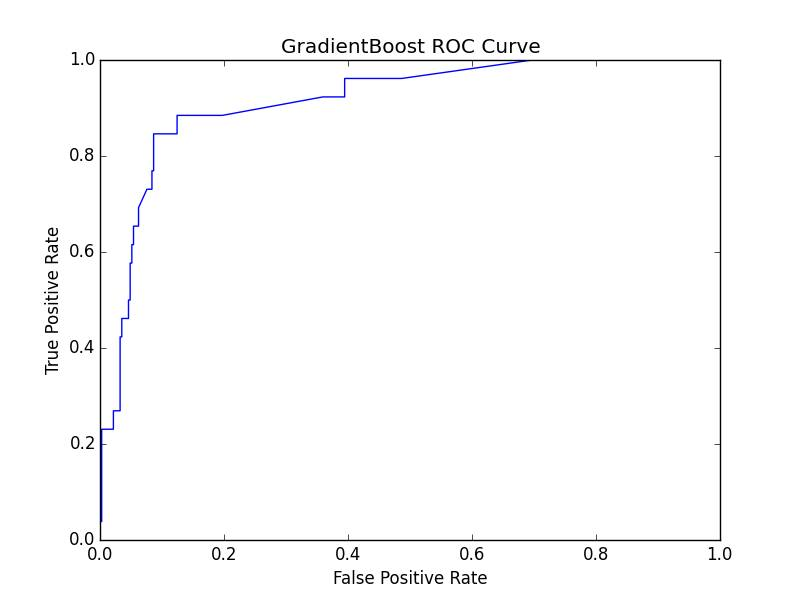
\includegraphics[scale=0.37]{img/grad_roc.jpg}}
\end{figure}

The following figures visualize the curve of AUC score against the number of
estimators for the random forest and gradient boosting classifiers. The random
forests classifiers appeared to increase as the number of estimators increased.
However, similar to the SVMs, this increase tapered off and the improvement
slowed as the number of estimators went up.

\begin{figure}[h]
    \centering
    \subfloat[Random forest]{{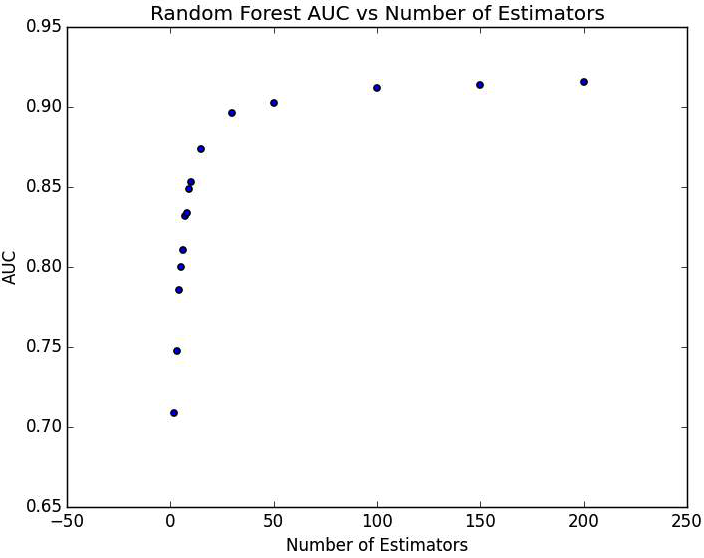
\includegraphics[width=6.5cm]{img/forest_auc_est.jpg} }}
    \qquad
    \subfloat[Gradient boosting]{{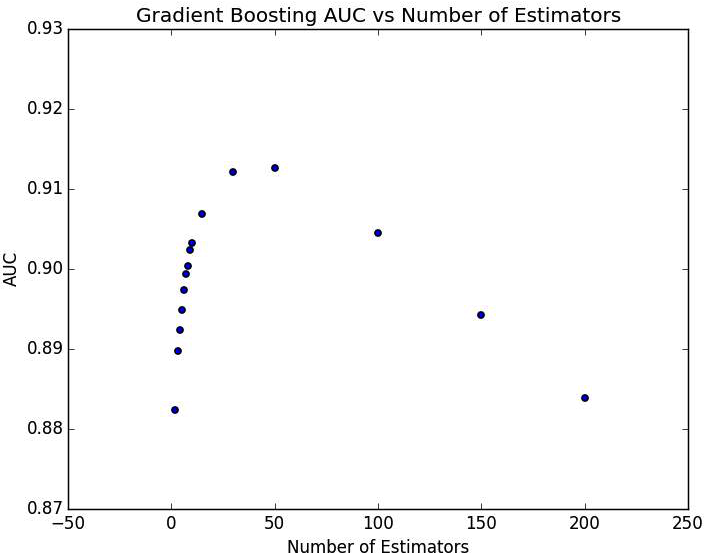
\includegraphics[width=6.5cm]{img/grad_auc_est.jpg} }}
\end{figure}

We still wanted to see whether we could improve the model.
With inspiration from the Bagging classifier, which trains multiple trees based
on subsets of the data and then votes, we tried to combine our models in a
similar way by training multiple trees based on the entire dataset and then
voting.  The hope here was that there was a good enough mix in the correctness
to make this a viable method.  However, when we made multiple of the same
estimator, it did not achieve good performance.  It ended up being inconsistent
and it was hit-or-miss whether it would beat the gradient boosting classifier.
The AUCs achieved over multiple runs of multiple Adaboost instances, as well as
those achieved with a combination of ensembles are shown below.\\

\begin{tabular}{c|ccccc}
\# Adaboost Instances & 1 & 3 & 5 & 7 & 9\\
\hline
Run 1 & \textbf{0.9094} & 0.9093 & 0.9093 & 0.9093 & 0.9094\\
Run 2 & 0.9110 & 0.9110 & 0.9111 & \textbf{0.9112} & 0.9111\\
Run 3 & \textbf{0.9109} & 0.9108 & 0.9109 & 0.9108 & 0.9108
\end{tabular}

\begin{tabular}
{c|cccccc}
Estimator & All 5 & Adaboost & Gradient Boosting & Random Forest & Bagging & Extra Trees\\
\hline
Run 1 & \textbf{0.9106} & 0.8953 & 0.9097 & 0.9051 & 0.8896 & 0.9028\\
Run 2 & 0.9114 & 0.8925 & \textbf{0.9132} & 0.9047 & 0.8937 & 0.9036\\
Run 3 & 0.9118 & 0.8921 & \textbf{0.9118} & 0.9065 & 0.8943 & 0.9049\\
Run 4 & 0.9137 & 0.8959 & \textbf{0.9149} & 0.9067 & 0.8932 & 0.9069
\end{tabular}

Given the inconsistency of our own boosting method, we felt that we did not have
sufficient evidence to prove its performance, even though it occassionally did
outperform our individual ensembles.

Another method we tried was using estimators other than decision trees as the
base estimators in the ensemble functions, like SVMs instead of decision trees.
However, not only did the training time increase significantly, but the results
also suffered. These are displayed in the figure below.

\begin{tabular}
{c|cccccc}
Estimator & N=3 & 5 & 7 & 9 & 15 & 30\\
\hline
SVM & 0.7986 & 0.7646 & 0.7526 & 0.7494 & 0.7469 & 0.7462\\
Decision Tree & 0.8759 & 0.8861 & 0.8910 & 0.8938 & 0.8978 & 0.8913
\end{tabular}

\subsection{Kaggle Winner: ``Small Yellow Duck"}

To evaluate the success of our project, we compared ourselves to a professional data scientist who won second place in the Kaggle Competition \cite{SYD}.
This data scientist goes by the name ``Small Yellow Duck".
She chose a classification model that takes the average of the probabilities predicted by five instances of the Random Forest Classifier, which is an ensemble learning method that constructs multiple decision trees to create a stronger classification model.

Small Yellow Duck first makes a couple of observations before implementing feature extraction.
First, she observes human bidding activity tends to peak daily as seen in Figure 7. %this figure number might change
Over the course of three days, there are three peaks where human bidding activity is higher.
She theorizes that this may be because of auctions ending at the same time everyday.

%\clearpage

\begin{figure}[h]
\centering
\captionbox{Daily peaks of human bidding activity}{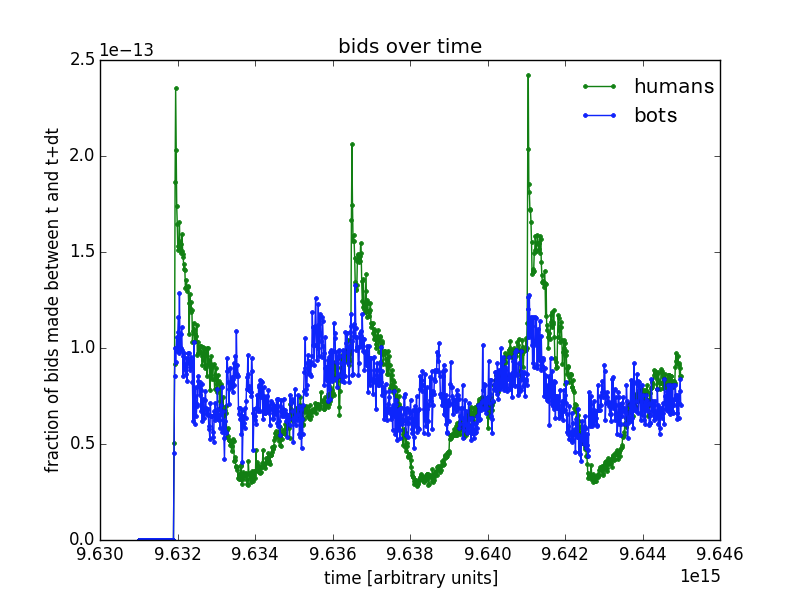
\includegraphics[scale=0.26]{img/yellowduck1.png}}
\end{figure}

Another observation she made is that auctions tend to last for longer than two weeks.
In this timeframe, robots do not place any bids between 11 to 14 days before the auction ends.
In Figure 8, the auction runs for approximately 17 days. %might need to change figure number
For some reason, between days 11 and 14, human bidding commences while bots tend to keep silent in this duration.

\begin{figure}[h]
\centering
\captionbox{Time Duration of Auction}{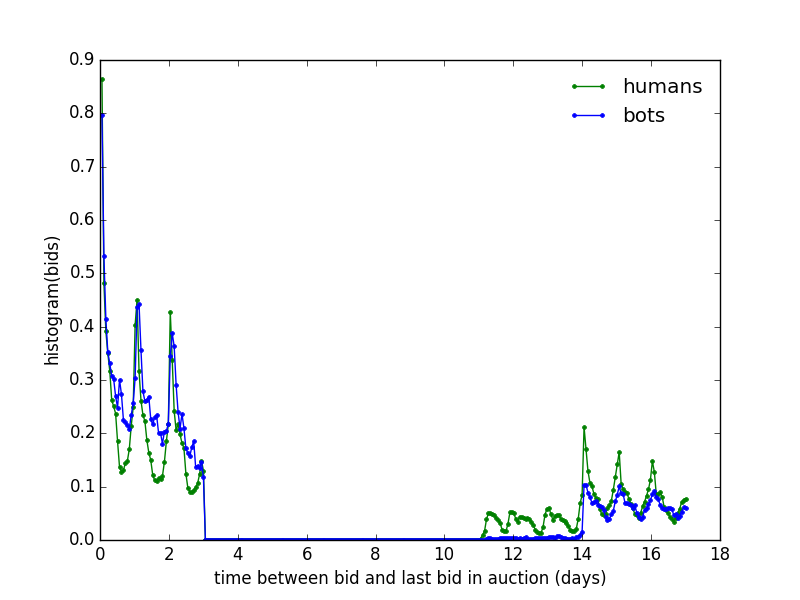
\includegraphics[scale=0.26]{img/yellowduck2.png}}
\end{figure}

During feature extraction, Small Yellow Duck was able to extract temporal features such as the median time between user's bid and user's previous bid and min and median times between a user's bid and previous bid by another user in the same auction.
She was also able to extract spatial features such as the mean number of bids a user made per auction, entropy for how many bids a user placed on each day of the week, max number of bids in a 20 min span, total number of bids placed by user, average number of bids a user placed per URL, and number of bids placed by the user on each of three weekdays in the data.

In order to evaluate her results, Small Yellow Duck does cross validation with 100 different training and validation splits where 80\% was training data and 20\% was validation data.
In terms of runtime, training and predicting takes around 3 minutes while 100-fold cross-validation takes around 20 minutes on Mac OSX with a 2.7 GHz Intel Core i5 processor and 8GB of RAM.
As a result, the AUC score tends to average at 0.94167. 

\section{Discussion}

In conclusion, we started this project by comparing and contrasting different algorithms.
Additionally, we pre-preprocessed and tested various combinations of the provided features.
In the end, we were pleased to produce results comparable to the Kaggle winner's approach and high enough to be in the top 15\% of the leaderboard.
The optimal algorithms turned out to be gradient boosting and other boosting machine learning approaches.

From this project, we gained a few takeaways and future directions.
First of all, manipulating a lot of data can be difficult, but using the right tools, finding the right features, organizing/sorting it beforehand, or storing them as binaries make a huge difference.
Secondly, temporal features are not nearly as powerful as we originally thought.
Once we added entropy terms and different metrics for the number of resources each user was using to bid, we did see dramatic improvement.
Although our results are comparable, there are potentially better features that could be processed.

Furthermore, as state-of-the-art as certain algorithms are, we should never underestimate the power of numbers.
Combining multiple estimators through different boosting methods allows an estimator to fill in the gaps where another estimator might fail, making for a more powerful classification algorithm.
Although boosting the algorithms greatly improves performance, we would have liked to seen if there was a singular algorithm that is just as powerful on its own without taking too much training time.
Also, we did attempt a group-based and graph-based approach to apply to our data set; however, the scalability proved to be a huge issue.
Group-based were difficult to debug in the time we needed for this project because of its high complexity.
In addition, even though graph-based approach is scalable when data is in a graph form, it is not scalable when preprocessing data into a graph form.
In conclusion, we learned quite a lot of interesting ways to manipulate large amounts of data and get important features out of our data set.
In addition, we were able to make a good analysis of what types of algorithms performed better than others and which features contribute the most in improving the performance of our algorithms.

\section{Contributions}

Daniel: Report

Meghana: Presentation, Wrote up Kaggle winner code portion, Report

Sara: Implemented BIRDNEST, Presentation, Report

Sonu: Presentation, Attempted EdgeCentric 

Andrew: Implemented Machine learning code, Presentation, Report, Attempted ND-SYNC

\begin{thebibliography}{123}

\bibitem{auction} Auction Sniping. Wikimedia Foundation, n.d. Web. 1 Mar. 2016.
\bibitem{ndsync} Giatsoglou, M. et. al. ``ND-Sync: Detecting Synchronized Fraud Activities." Advances in Knowledge Discovery and Data Mining, 2015, 201-214t
\bibitem{glad} Qi, Y., Xinran He, and Yan Liu. ``GLAD: Group Anomaly Detection in Social Media Analysis- Extended Abstract." arXiv:1410.1940.
\bibitem{birdnest} Hooi, B., et. al. ``BIRDNEST: Bayesian Inference for Ratings-Fraud Detection." arXiv:1511.06030
\bibitem{rsc} Costa, A.F. et. al. ``RSC: Mining and Modeling Temporal Activity in Social Media." Proceedings of the 21th ACM SIGKDD International Conference on Knowledge Discovery and Data Mining, 2015, pp. 269-278
\bibitem{sfp} Vaz de Melo, P. et. al. ``The Self-Feeding Process: A Unifying Model for Communication Dynamics in the Web." Proceedings of the International Conference on World Wide Web (WWW), pp. 1319?1330, 2013.
\bibitem{cicp} Malmgren, M.D. et. al. ``Characterizing Individual Communication Patterns." Proceedings of the 15th ACM SIGKDD International Conference on Knowledge Discovery and Data Mining, 2009, pp. 607?616.
\bibitem{edgecentric} Shah, N. et. al. ``EdgeCentric: Anomaly Detection in Edge-Attributed Networks." arXiv:1510.05544.
\bibitem{SYD} ``Facebook IV Winner's Interview: 2nd Place, Kiri Nichol(aka Small Yellow Duck)." No Free Hunch. N.p., 19 June 2015. Web. 1 Mar. 2016.

\end{thebibliography}

\end{document}
